\chapter{Building large SpiNNaker machines}
	
	Like any super computer, physically putting together a large SpiNNaker
	machine poses many challenges in terms of organisation, assembly and
	maintainance. One of the key tasks in this process is the installation of
	network cables such that a desired overall network topology is constructed.
	The largest planned SpiNNaker machine will use \num{3600} S-ATA
	\cite{sata3spec} cables to interconnect its \num{1200} circuit boards,
	creating a hexagonal torus topology. Since the machine will be installed
	within standard server room cabinets (which are not available in a
	giant-doughnut form-factor) a mapping from a board's logical location in the
	network topology to its physical location must be constructed. In addition,
	the interconnect technology employed by SpiNNaker restricts the length of
	S-ATA cables used to $\le$~\SI{1}{\meter}, constraining the possible mappings
	used. In addition the practical issues of installation complexity and
	maintainance must be considered since all \num{3600} cables must ultimately
	be installed and maintained by human operators.
	
	In this chapter I describe a novel technique for physically laying out
	machines configured in hexagonal torus topologies, such as SpiNNaker, in
	commercial machine rooms, building on the techniques used in more
	conventional torus topologies. In addition, I also propose a new methodology
	for installing and maintaining super computer cabling which which exploits
	existing diagnostic features of the SpiNNaker hardware to interactively guide
	and validate cable installation. Finally, I demonstrate how these new
	techniques have been used successfully to interconnect a prototype
	\num{518400} core SpiNNaker machine in substantially less time than the
	industry norm.
	
	In this chapter, the term \emph{unit} refers to the smallest physical
	ecomponent between which connections connections are to be made. For example,
	in a SpiNNaker machine a unit is a 48-chip board while in data center, a unit
	might be a server blade.
	
	\section{Related work}
		
		In this section I describe the techniques conventionally employed when
		laying out and interconnecting the units within super computers. Due to
		SpiNNaker's hexagonal torus topology and dense physical packing of units,
		these existing techniques are found to be insufficient. In the remainder of
		the chapter we will explore solutions to the limitations exposed below.
		
		\subsection{Avoiding long cables}
			
			Na\"ive arrangements of torus topologies, including hexagonal torus
			topologies, feature long `wrap-around' connections which connect units at
			the peripheries of the system. These connections can be problematic for
			numerous reasons:
			
			\begin{description}
				
				\item[Performance] Signal quality diminishes as cables get longer,
				requiring the use of slower signalling speeds, increased error
				correction overhead or more complex hardware.
				
				\item[Energy] Longer cables require higher drive strengths and/or
				buffering to maintain signal integrity.
				
				\item[Cost] Cost Shorter cables are cheaper than long ones.  Longer
				cables imply more wire in a given space making the tasks of routing or
				cable installation more difficult increasing labour costs by as much as
				$5\times$ \cite{curtis12}.
				
			\end{description}
			
			In conventional torus topologies the need for long cables is eliminated
			by folding and interleaving units of the network \cite{dally04}. For
			example, for a 1D torus topology (a ring network), one long connection
			exists to connect the two opposite sides of the system. To remove these
			long connections, half the units are `folded' on top of the others and
			then this arrangement of units is interleaved as illustrated in figure
			\ref{fig:ring-folding}.
			
			\begin{figure}
				\center
				\begin{subfigure}[b]{0.39\linewidth}
					\center
					\buildfig{figures/ring-folding-row.tex}
					\caption{A ring network}
					\label{fig:ring-folding-row}
				\end{subfigure}
				\begin{subfigure}[b]{0.24\linewidth}
					\center
					\buildfig{figures/ring-folding-folded.tex}
					\caption{Folded}
					\label{fig:ring-folding-folded}
				\end{subfigure}
				\begin{subfigure}[b]{0.35\linewidth}
					\center
					\buildfig{figures/ring-folding-interleaved.tex}
					\caption{Folded and interleaved}
					\label{fig:ring-folding-interleaved}
				\end{subfigure}
				
				\caption{Folding and interleaving a ring network to reduce maximum wire
				length.}
				\label{fig:ring-folding}
			\end{figure}
			
			Folding and interleaving has the effect of approximately doubling the
			average cable length but also eliminates the need for a cable spanning
			the entire system. Since the mean cable length is typically already
			short, doubling it in exchange for a substantially reduced maximum cable
			length is often preferable.
			
			The folding and interleaving process may be extended to $N$-dimensional
			torus topologies by folding each dimension in turn. Since all dimensions
			are orthogonal, the folding process only moves units in the dimension
			being folded. In the hexagonal torus topology, however, the three
			dimensions are non-orthogonal and thus folding in one dimension also
			moves units in other dimensions, preventing the edges of the torus
			meeting as illustrated in figure \ref{fig:failing-to-fold-hex-toruses}.
			
			\begin{figure}
				\center
				\begin{subfigure}[b]{0.24\linewidth}
					\center
					\buildfig{figures/failing-to-fold-hex-toruses-none.tex}
					\caption{Not folded}
					\label{fig:failing-to-fold-hex-toruses-none}
				\end{subfigure}
				\begin{subfigure}[b]{0.24\linewidth}
					\center
					\buildfig{figures/failing-to-fold-hex-toruses-x.tex}
					\caption{X}
					\label{fig:failing-to-fold-hex-toruses-x}
				\end{subfigure}
				\begin{subfigure}[b]{0.24\linewidth}
					\center
					\buildfig{figures/failing-to-fold-hex-toruses-y.tex}
					\caption{Y}
					\label{fig:failing-to-fold-hex-toruses-y}
				\end{subfigure}
				\begin{subfigure}[b]{0.24\linewidth}
					\center
					\buildfig{figures/failing-to-fold-hex-toruses-z.tex}
					\caption{Z}
					\label{fig:failing-to-fold-hex-toruses-z}
				\end{subfigure}
				
				\caption{Schematics showing hexagonal torus topologies folded along
				each of their non-orthogonal dimensions. Note that folding along
				the Z axis brings the \emph{wrong} edges closer together.}
				\label{fig:failing-to-fold-hex-toruses}
			\end{figure}
		
		\subsection{Cabling installation}
			
			Existing machine room installations feature very repetitive cabling
			patterns which can easily be memorised by a human technician. For example
			in BlueGene super computers the connectivity between units is highly
			regular \cite{lakner07} while in data centre networks cabling often
			centres around a small number of high-port-count switches
			\cite{cisco07,csernai15}. Cable installation is usually only aided by
			the labelling of connectors and sockets in a standardised manner
			\cite{tia2006} such as in figure \ref{fig:bgWiring}.
			
			\begin{figure}
				\center
				\begin{subfigure}[t]{0.5\textwidth}
					\begin{tikzpicture}
						\node (cables) [inner sep=0]
						      {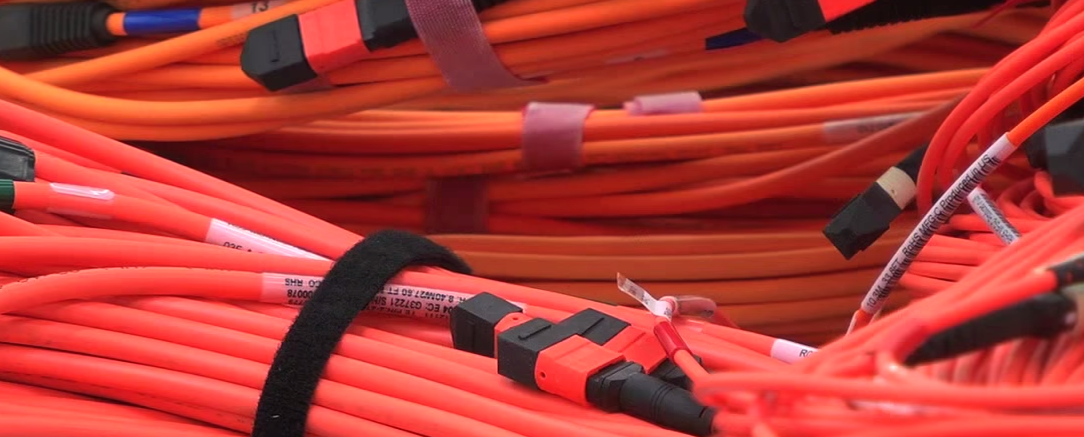
\includegraphics[width=\textwidth]{figures/bgCables.png}};
						\node (sockets) [inner sep=0, below=1.0em of cables]
						      {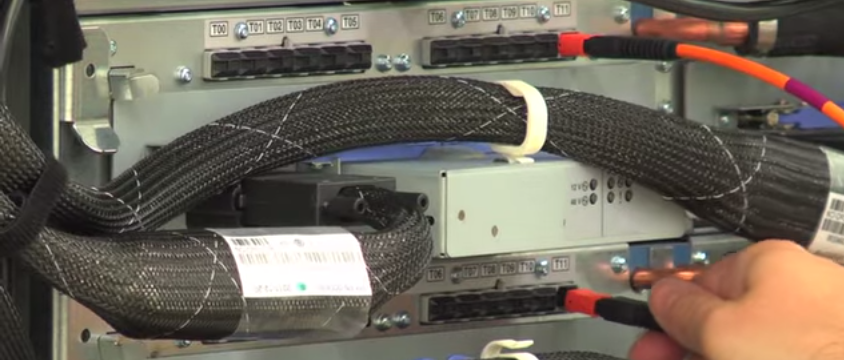
\includegraphics[width=\textwidth]{figures/bgSockets.png}};
						
						% Point at label on cable
						\draw [white, <-, line width=0.4em]
						      ([shift={(0.7cm, -0.3cm)}]cables.center)
						      -- ++(45:1cm);
						
						% Point at label on socket
						\draw [white, <-, line width=0.4em]
						      ([shift={(-1.0cm, 1.1cm)}]sockets.center)
						      -- ++(-45:1cm);
					\end{tikzpicture}
					
					\caption{Pre-labelled cables and sockets}
					\label{fig:bgWiringLabels}
				\end{subfigure}
				~
				\begin{subfigure}[t]{0.30\textwidth}
					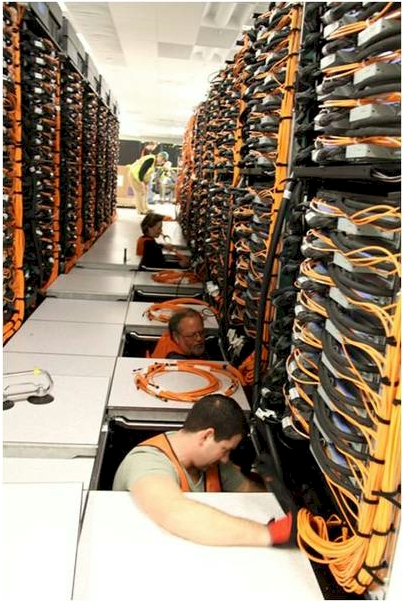
\includegraphics[height=6.15cm]{figures/bgWiring.jpg}
					
					\caption{Installation of cables}
					\label{fig:bgWiringInstallation}
				\end{subfigure}
				
				\caption{BlueGene/Q cable installation \cite{cscs13}}
				\label{fig:bgWiring}
			\end{figure}
			
			Despite the regularity and careful labelling of cables, the cost of
			installation and maintenance alone can be significant with costs in the
			range of \$45-95 per \SI{1}{\meter} cable run and \$100-400 for runs of
			\SI{10}{\meter} reported in the literature \cite{mudigonda11}. Much of
			this cost is due to the care required during installation to avoid
			miswiring and ensure that cooling airflow is not hampered by cable runs
			\cite{cisco07}.
			
			Many researchers have attempted to control cable installation costs by
			trying to reduce the number or length of cables required by developing
			alternative network topologies \cite{curtis12, popa10, mudigonda11}.
			Unfortunately, these techniques do not apply to SpiNNaker since its
			network topology is fixed.
			
			Some super computers make use of large custom `midplane` PCBs in place of
			cables to interconnect units within a cabinet and thus simplify the task
			of cable installation \cite{prickett10}. This scheme can greatly reduce
			wiring complexity since only coarser-grain cabinet-to-cabinet
			connectivity is provided by cables. Unfortunately this technique is
			expensive and also constrains the dimensions of the network topology
			supported by the machine. Since the SpiNNaker platform is designed to
			scale from desktop machines to machine-room installations, this scheme is
			not practical.
	
	\section{Folding \& interleaving hexagonal toruses}
		
		The first step towards a practical machine-room installation of a large
		machine using a hexagonal torus topology is to find an arrangement of
		boards between which cable lengths are minimised. In this section I
		describe a sequence of transformations which map the positions of units in
		a hexagonal torus topology onto a regular rectangular grid which may be
		folded and interleaved to eliminate long wires. It is worth emphasising
		that this transformation only affects the \emph{physical} positions of
		units and \emph{not} their connectivity.
		
		As described earlier in \S\ref{sec:parititioning} (page
		\pageref{sec:parititioning}), hexagonal torus topologies may be partitioned
		into units containing wrapped-triples of nodes. For example, in SpiNNaker,
		chips (nodes) are partitioned into circuit boards (units) containing 48
		chips. For completeness, this section describes the process of folding both
		systems whose units are individual nodes and those whose units are
		wrapped-triples.
		
		The transformation process is divided into two parts, each described
		separately in this section.
		
		\begin{description}
			
			\item[Parallelogram to rectangle] Units of the system are transformed
			from a parallelogram shape to a rectangular shape.
			
			\item[Uncrinkle] Units within the rectangle are moved such that they all
			lie on a regular (and fully packed) 2D grid.
			
		\end{description}
		
		\subsection{Parallelogram to rectangle}
			
			The hexagonal torus topology is most naturally drawn as a parallelogram
			as illustrated in figures \ref{fig:hex-to-plane-node-native} and
			\ref{fig:hex-to-plane-native}. Two transformations are presented which
			transform these arangements of units into a rectangular form: shearing
			and slicing.
			
			A \SI{30}{\degree} shear transformation distorts networks such that the X
			and Y axes become orthogonal leading to a rectangular arrangement of
			units as illustrated in figures \ref{fig:hex-to-plane-node-shear} and
			\ref{fig:hex-to-plane-shear}.
			
			The slice transformation slices the units protruding from the
			left-hand-side of the parallelogram and moves them into the matching gap
			on the opposite side of the parallelogram as illustrated in figures
			\ref{fig:hex-to-plane-node-slice} and \ref{fig:hex-to-plane-slice}.
			 
			While the shear transformation introduces some distortion causing cables
			in the Z dimension to become $\sqrt{2}\times$ longer it leaves the
			pattern of wrap-around connections remains unchanged. By contrast, the
			slice transformation does not elongate any cables but changes the pattern
			of wrap-around connections. The exact pattern wrap-around connections
			produced when slicing depends on the aspect ratio of the network as
			illustrated in \ref{fig:slicing-examples} and influences the choice of
			folding technique applied as described later.
			
			\begin{figure}
				\center
				\begin{subfigure}[b]{0.32\linewidth}
					\center
					\buildfig{figures/hex-to-plane-node-native.tex}
					
					\caption{$7 \times 7$ node torus}
					\label{fig:hex-to-plane-node-native}
				\end{subfigure}
				\begin{subfigure}[b]{0.32\linewidth}
					\center
					\buildfig{figures/hex-to-plane-node-shear.tex}
					
					\caption{Sheared}
					\label{fig:hex-to-plane-node-shear}
				\end{subfigure}
				\begin{subfigure}[b]{0.32\linewidth}
					\center
					\buildfig{figures/hex-to-plane-node-slice.tex}
					
					\caption{Sliced}
					\label{fig:hex-to-plane-node-slice}
				\end{subfigure}
				
				\caption{Transformations of hexagonal toruses of nodes into a
				rectangular form. Thin lines show wrap-around links. Pointy-topped
				hexagons represent individual nodes.}
				\label{fig:hex-to-plane-node}
			\end{figure}
			
			\begin{figure}
				
				\begin{subfigure}[b]{0.32\linewidth}
					\center
					\buildfig{figures/hex-to-plane-native.tex}
					
					\caption{$4 \times 4$ triad torus}
					\label{fig:hex-to-plane-native}
				\end{subfigure}
				\begin{subfigure}[b]{0.32\linewidth}
					\center
					\buildfig{figures/hex-to-plane-shear.tex}
					
					\caption{Sheared}
					\label{fig:hex-to-plane-shear}
				\end{subfigure}
				\begin{subfigure}[b]{0.32\linewidth}
					\center
					\buildfig{figures/hex-to-plane-slice.tex}
					
					\caption{Sliced}
					\label{fig:hex-to-plane-slice}
				\end{subfigure}
				
				\caption{Transformations of hexagonal toruses of wrapped triples into a
				rectangular form.  Thin lines show wrap-around links. Flat-topped
				hexagons represent a wrapped triple of nodes.}
				\label{fig:hex-to-plane}
			\end{figure}
			
			\begin{figure}
				\center
				\buildfig{figures/slicing-examples.tex}
				\caption{Patterns of wiring in sliced systems of various sizes.}
				\label{fig:slicing-examples}
			\end{figure}
			
		\subsection{Uncrinkling}
			
			Though the transformmation step yields rectangular arrangements of units,
			these arrangements do not fall onto a regular 2D grid, with the exception
			of the shear transform on individual nodes. Figure \ref{fig:uncrinkling}
			illustrates how the various arrangements of hexagons may be moved to
			`uncrinkle' the units into a regular grid.
			
			\begin{figure}
				\center
				\begin{subfigure}[b]{0.44\linewidth}
					\center
					\buildfig{figures/uncrinkling-node-sheared.tex}
					
					\caption{$7 \times 7$ nodes, sheared}
					\label{fig:uncrinkling-node-sheared}
				\end{subfigure}
				\begin{subfigure}[b]{0.44\linewidth}
					\center
					\buildfig{figures/uncrinkling-node-sliced.tex}
					
					\caption{$7 \times 7$ nodes, sliced}
					\label{fig:uncrinkling-node-sliced}
				\end{subfigure}
				
				\vspace{1cm}
				
				\begin{subfigure}[b]{0.44\linewidth}
					\center
					\buildfig{figures/uncrinkling-sheared.tex}
					
					\caption{$4 \times 4$ triples, sheared}
					\label{fig:uncrinkling-sheared}
				\end{subfigure}
				\begin{subfigure}[b]{0.44\linewidth}
					\center
					\buildfig{figures/uncrinkling-sliced.tex}
					
					\caption{$4 \times 4$ triples, sliced}
					\label{fig:uncrinkling-sliced}
				\end{subfigure}
				
				\vspace{1em}
				
				\caption{Mapping rectangular arrangements of units into a square grid.
				Thick lines show how layers of units are uncrinkled.  Annotations show
				how the relative positions of nodes and wrapped triples change after
				uncrinkling.}
				\label{fig:uncrinkling}
			\end{figure}
			
			In the figure, the numbered units enumerate the different positions on
			the crinkle and those labelled alphabetically are those that immediately
			surround them. From this we can observe that uncrinkling largely
			preserves spatial locality but some distortion is introduced, separating
			previously neighbouring units. For example, in figure
			\ref{fig:uncrinkling-sheared}, the units labelled `1' and `i' are
			neighbours before uncrinkling but are separated by a (Euclidean) distance
			of $\sqrt{5}$ afterwards. Note that the distortion introduced depends on
			what part of the crinkle is considered, for example `2' and `a' have
			distance 2 but are logically connected in the same way.
		
		\subsection{Folding and Interleaving}
			
			Once a regular grid of units has been formed, this may be folded in the
			conventional way, eliminating long cables crossing from left-to-right and
			top-to-bottom as illustrated in \ref{fig:folding-sheared}.
			
			Unfortunately, for sliced systems whose dimensions are not of the ratio
			$1:2$, the pattern of wrap-around cables may also include some cables
			which do not cross directly to the opposite side of the system (refer
			back to figure \ref{fig:slicing-examples}). As a result of these
			connections, folding does not successfully eliminate all long
			connections. An exception to this rule is sliced systems whose dimensions
			are in the ratio $1:1$ where folding twice along the Y axis may
			successfully eliminate all wrap-around connections as illustrated in
			\ref{fig:folding-sliced}.
			
			\begin{figure}
				\begin{subfigure}{\linewidth}
					\center
					\buildfig{figures/folding-sheared.tex}
					\caption{$N \times M$ sheared systems and $N \times 2N$ sliced systems}
					\label{fig:folding-sheared}
				\end{subfigure}
				
				\vspace{1em}
				
				\begin{subfigure}{\linewidth}
					\center
					\buildfig{figures/folding-sliced.tex}
					\caption{$N \times N$ sliced systems}
					\label{fig:folding-sliced}
				\end{subfigure}
				
				\caption{Schematic illustrating elimination of long wrap-around links
				during folding. In each example a single link has been highlighted to
				aid in following the process.}
				\label{fig:folding}
			\end{figure}
			
			Once folded, the 2D grid is straight-forwardly interleaved as illustrated
			previously in figure \ref{fig:ring-folding}. The interleaving process
			introduces some additional distortion to the layout of units and causes
			most connections to become twice as long. For sliced $1:1$ systems, the
			additional fold results in additional overhead during interleaving since
			four layers of the system are interleaved.
		
		\subsection{Mapping to Cabinets}
			
			In the final step of the process is to map the 2D grid of units into
			positions in machine room cabinets as illustrated in figure
			\ref{fig:million-core-machine}. As illustrated in figure
			\ref{fig:cabinetisation}, first the grid of units is partitioned into
			groups of columns, one per cabinet, then groups of rows one per frame per
			cabinet. The units in each group are then allocated to slots within a
			frame, interleaving the rows of the groups as shown.
			
			\begin{figure}
				\center
				\buildfig{figures/cabinet-units.tex}
				
				\caption{An illustration of the physical construction of a
				multi-cabinet SpiNNaker system. (Note: network cables \emph{not}
				installed.)}
				\label{fig:cabinet-units}
			\end{figure}
			
			\begin{figure}
				\center
				\buildfig{figures/cabinetisation.tex}
				
				\caption{Mapping from 2D space to cabinets, frames and boards.}
				\label{fig:cabinetisation}
			\end{figure}
		
	\section{Cable installation}
		
		Cable installation is performed by a team of (human) technicians who must
		ensure that all network cables are correctly installed. As illustrated in
		previously in figure \ref{fig:cabinet-units}, the density of SpiNNaker's
		units, combined with the nature of the hexagonal torus topology, poses a
		challenge. To address this challenge I propose a semi-automated approach to
		cable installation which exploits diagnostic facilities available in the
		majority of super computers in order to guide technicians through the
		cabling process, interactively guiding installation and maintenance.
		
		\subsection{Interactive technician guidance and validation}
			
			While automated systems for validating cabling correctness are
			commonplace, these systems are typically used only after cabling has been
			completed \cite{lakner07}. As with other large-scale machines, SpiNNaker
			includes a low-bandwidth system management bus which may be used to
			interrogate network hardware and control diagnostic LEDs prior to the
			installation of the main SpiNNaker network interconnect.  Using these
			facilities I have constructed a tool called SpiNNer which interactively
			guides a technician, or team of technicians, through the cable
			installation process, validating each connection in real-time.
			
			Diagnostic LEDs mounted on each SpiNNaker board (figure
			\ref{fig:interactive-wiring-guide-leds}) are used to indicate the
			endpoints of the cable currently being installed. Simultaneously a
			Text-To-Speech (TTS) system gives an audible indication of which cable
			type is to be used and location of each connection.  Additionally, a GUI
			via a computer display (figure \ref{fig:interactive-wiring-guide-gui}).
			The centre of the display shows a `big-picture' perspective of the
			locations of the boards to be connected. The detailed views on the left
			and right indicate which of the six sockets on each board the cables
			should connect.
			
			\begin{figure}
				\center
				\begin{subfigure}[b]{0.40\textwidth}
					\begin{tikzpicture}
						\node (leds) [inner sep=0]
						      {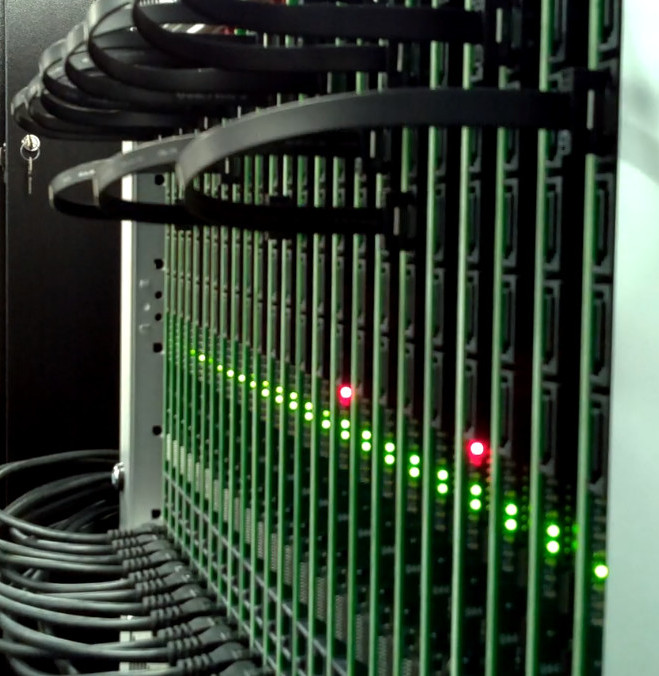
\includegraphics[width=\textwidth]{figures/leds.jpg}};
						% Point at left LED
						\draw [white, <-, line width=0.4em]
						      ([shift={(-0.0cm, -0.6cm)}]leds.center)
						      -- ++(225:1cm);
						% Point at right LED
						\draw [white, <-, line width=0.4em]
						      ([shift={(1.1cm, -1.1cm)}]leds.center)
						      -- ++(225:1cm);
					\end{tikzpicture}
					
					\caption{Diagnostic LEDs}
					\label{fig:interactive-wiring-guide-leds}
				\end{subfigure}
				~
				\begin{subfigure}[b]{0.546\textwidth}
					\begin{tikzpicture}[thin, black!20!white]
						\node (screen) [inner sep=0]
						      {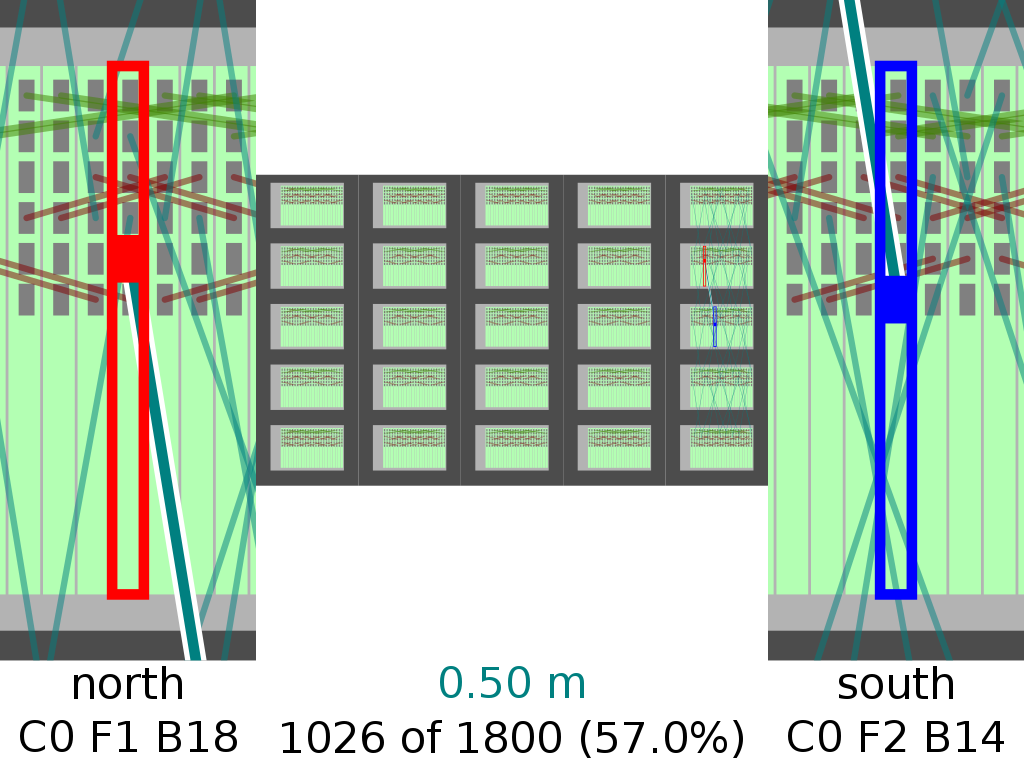
\includegraphics[width=\textwidth]{figures/wiring_guide_screenshot.png}};
						\draw (screen.south west) rectangle (screen.north east);
					\end{tikzpicture}
					
					\caption{Interactive wiring guide GUI}
					\label{fig:interactive-wiring-guide-gui}
				\end{subfigure}
				
				\caption{The SpiNNer interactive wiring guide uses a GUI,
				text-to-speech and diagnostic LEDs to assist during cable
				installation.}
				\label{fig:interactive-wiring-guide}
			\end{figure}
			
			SpiNNer also validates the connectivity of the system in real-time by
			polling the diagnostic interfaces of the network hardware at the
			endpoints of the cable being installed to determine if they are correctly
			connected. If a miswiring occurs, this is immediately detected and
			announced via TTS enabling the technician to immediately correct the
			error. Once a cable has been installed correctly, the software
			automatically advances to the next cable meaning direct interaction with
			the software by the technician is minimal. In practice, it is rarely
			necessary to refer to the GUI.
		
			SpiNNer presents the cables in an order intended to maximise ease of
			installation. Cables are installed in three groups with intra-frame
			cables being installed first, followed by intra-cabinet cables and
			inter-cabinet cables. Within each group, the tightest cables are
			installed first resulting in slacker cables naturally being installed
			over the top of already installed cables. By grouping cables in this
			manner, multiple technicians may work independently on the wiring within
			individual frames and cabinets.
			
			SpiNNer may also be used to repair or replace cables in the system.
			During maintenance, obstructing cables may be blindly removed alongside
			any cable being replaced. At the conclusion of the process, the wiring
			guide may be used to interactively guide re-installation of all removed
			cables.
		
		\subsection{Cable selection}
			
			Controlling slack is critical to ensuring reliable and maintainable
			cabling installations. If cables are too tight, cables and connectors can
			become easily damaged and when too slack, the excess cable obstructs
			other cables and can easily become tangled and damaged \cite{cisco07}. It
			has been observed that when ready-made cables are employed technicians
			frequently over-estimate the cable lengths required preferring to use
			overly long cables for all connections \cite{mazaris97}. To solve this
			problem, the SpiNNer wiring guide software dictates the cable lengths to
			be used by an installer based the rule of (three-)thumbs according to
			Mazaris \cite{mazaris97}. This rule suggests that an ideal amount of
			slack is approximately that which can be wrapped around three fingers.
			Specifically, the shortest available cable is selected which ensures at
			least \SI{5}{\centi\meter} of slack.
			
			The SpiNNer tool allocates cables assuming all cables take a Euclidean
			straight-line path between the endpoints of the connection. The result is
			that wiring is not routed through dedicated cable management structures
			but is simply suspended by its connectors in front of the machine. As
			demonstrated later, this unconventional approach leads neither to cooling
			problems nor increased maintenance effort.
	
	\section{Results and Evaluation}
		
		This stuff has been used and works. In this section I'll go over the
		overheads introduced by the various transformations and
		folding/interleaving steps and show a wiring scheme for a large machine
		which uses only short cables. I'll then show how SpiNNer was used to
		install this wiring plan into a very large machine without foobaring the
		cooling and in very little time. I'll also report on difficulty of
		maintenance.
		
		\subsection{Cable length}
			
			The transformation from regular hexagonal torus to a folded and
			interleaved form introduces some overhead to the cable lengths required.
			Using figure \ref{fig:uncrinkling} (page \pageref{fig:uncrinkling}), it
			is possible to compute the exact overhead introduced when each type of
			transformation proposed.
			
			For example, to compute the mean overhead introduced by the slicing
			technique when applied to units composed of wrapped triples, consider
			figure \ref{fig:uncrinkling-sliced}. The uncrinkling pattern used to
			transform this topology is a repeating pattern of two units, a pair of
			which have been labelled $1$ and $2$ respectively. Unit $1$ is
			immediately surrounded by six units labelled $a$, $b$, $c$, $2$, $g$ and
			$h$. Similarly, unit $2$ is surrounded by units $1$, $c$, $d$, $e$, $f$
			and $g$. Before the transformation, the distances, $D$, to each of these
			units is $1$ but after the transformation is applied, this is not always
			the case. Additionally, folding and interleaving introduce additional
			overhead. In this example, if the system is folded into $f_x$ columns and
			$f_y$ rows, the distances between previously neighbouring units become:
			
			\begin{equation*}
				\begin{aligned}[c]
					D_{1\,\leftrightarrow{}\,a} &= \sqrt{f_x^2 + f_y^2} \\
					D_{1\,\leftrightarrow{}\,b} &= f_y \\
					D_{1\,\leftrightarrow{}\,c} &= \sqrt{f_x^2 + f_y^2} \\
					D_{1\,\leftrightarrow{}\,2} &= f_x \\
					D_{1\,\leftrightarrow{}\,g} &= f_y \\
					D_{1\,\leftrightarrow{}\,h} &= f_x
				\end{aligned}
				\hspace{2cm}
				\begin{aligned}[c]
					D_{2\,\leftrightarrow{}\,1} &= f_x \\
					D_{2\,\leftrightarrow{}\,c} &= f_y \\
					D_{2\,\leftrightarrow{}\,d} &= f_x \\
					D_{2\,\leftrightarrow{}\,e} &= \sqrt{f_x^2 + f_y^2} \\
					D_{2\,\leftrightarrow{}\,f} &= f_y \\
					D_{2\,\leftrightarrow{}\,g} &= \sqrt{f_x^2 + f_y^2}
				\end{aligned}
			\end{equation*}
			
			From these values, the mean and maximum connection distances after
			folding and interleaving may be computed. Table
			\ref{tab:transform-overhead} gives the mean and maximum connection
			distances for each of the four transformations described in this chapter.
			
			\begin{table}
				\begin{subtable}[b]{\linewidth}
					\center
					\begin{tabular}{l c c}
						\toprule
						& Shear & Slice \\
						\addlinespace
						Nodes &
							$\frac{f_x + f_y + \sqrt{f_x^2 + f_y^2}}{3}$ &
							$\frac{f_x + f_y + \sqrt{f_x^2 + f_y^2}}{3}$ \\
						\addlinespace
						Triples &
							$\frac{7f_x + 3\sqrt{f_x^2 + f_y^2} + \sqrt{(2f_x)^2 + f_y^2}}{9}$ &
							$\frac{f_x + f_y + \sqrt{f_x^2 + f_y^2}}{3}$ \\
						\bottomrule
					\end{tabular}
					
					\caption{Mean}
					\label{tab:transform-overhead-mean}
				\end{subtable}
				
				\vspace{1em}
				
				\begin{subtable}[b]{\linewidth}
					\center
					\begin{tabular}{l c c}
						\toprule
						& Shear & Slice \\
						\addlinespace
						Nodes &
							$\sqrt{f_x^2 + f_y^2}$ &
							$\sqrt{f_x^2 + f_y^2}$ \\
						\addlinespace
						Triples &
							$\sqrt{(2f_x)^2 + f_y^2}$ &
							$\sqrt{f_x^2 + f_y^2}$ \\
						\bottomrule
					\end{tabular}
					
					\caption{Maximum}
					\label{tab:transform-overhead-max}
				\end{subtable}
				
				\caption{Overheads introduced when transforming unit positions onto a
				regular grid.}
				\label{tab:transform-overhead}
			\end{table}
			
			From these results it is evident that shearing and slicing networks
			whose units are nodes result in identical mean and maximum overhead in
			cable length when folded similarly. Since sliced networks may require
			folding more than once along each axis the shearing approach is
			preferable in general.
			
			For networks constructed from units of wrapped triples, the slicing
			approach suffers the same mean and maximum overhead has networks of
			nodes, and less overhead than shearing for the same number of folds. For
			systems with an aspect ratio of $1:2$ (where both slicing and shearing
			require $f_x = f_y = 2$), the slicing transformation yields lower mean
			and maximum overhead than shearing. For all other aspect ratios (where
			slicing requires a greater degree of folding) the shearing technique
			produces lower overhead. The recommended transformations for a given
			machine are thus given in table \ref{tab:transform-recommended}.
			
			\begin{table}
				\center
				\begin{tabular}{lcc}
					\toprule
					                         & $1:2$  & Other \\
					\addlinespace
					\multirow{2}{*}{Nodes}   & Either & Shear\\
					                         & \footnotesize $\mu\approx2.28 \quad \vee\approx2.83$
					                         & \footnotesize $\mu\approx2.28 \quad \vee\approx2.83$\\
					\addlinespace
					\multirow{2}{*}{Triples} & Slice  & Shear\\
					                         & \footnotesize $\mu\approx2.28 \quad \vee\approx2.83$
					                         & \footnotesize $\mu\approx3.00 \quad \vee\approx4.47$\\
					\bottomrule
				\end{tabular}
				
				\caption{Recommended transformation and folding scheme for different
				system types. $\mu$ and $\vee$ give the mean and maximum wire
				distortion introduced, respectively.}
				\label{tab:transform-recommended}
			\end{table}
			
			\begin{figure}
				\center
				\buildfig{figures/million-core-machine.tex}
				
				\caption{Cabling plan for a \num{1036800} core SpiNNaker
				machine's \num{3600} cables.}
				\label{fig:million-core-machine}
			\end{figure}
			
			Following folding and mapping to physical locations, the cabling plans
			for large machines require no large gaps to be spanned.  The largest
			planned SpiNNaker machine, illustrated in figure
			\ref{fig:million-core-machine}, will be \SI{6}{\meter} wide but the
			largest gap any cable must span is \SI{66}{\centi\meter}. This distance
			is well within the \SI{1}{\meter} allowed by the hardware and cables.
			
		\subsection{Installation practicality}
			
			\begin{table}
				\center
				\begin{tabular}{lrr@{$\,$}l}
					\toprule
						System & Number of Cables & \multicolumn{2}{r}{Installation time} \\
					\midrule
						24 boards  & \num{72}   & \num{10} & \si{\minute}         \\
						1 cabinet  & \num{360}  & \num{4}  & \si{\hour}$^\dagger$ \\
						2 cabinets & \num{720}  & \num{2}  & \si{\hour}           \\
						5 cabinets & \num{1800} & ?        &                      \\
					\bottomrule
				\end{tabular}
				
				\caption{Installation times for various sizes of machine.
				$\dagger$~This machine was installed without real-time validation of
				connectivity.}
				\label{tab:install-time}
			\end{table}
			
			A number of SpiNNaker machines of various scales have been assembled
			using the techniques described in this chapter ranging from single frames
			of 24 boards to a half-scale 5 cabinet machine. Table
			\ref{tab:install-time} gives the reported installation times of each of
			these machines.
			
			The single cabinet machine's installation time is notably
			disproportionate to its size. When this system was assembled, real-time
			connection validation was not yet available. As a result, though cable
			installation was rapid correcting errors was extremely costly, requiring
			careful retracing of many installation steps.
			
			TODO: TALK ABOUT MULTI-PERSON-WIRING IN PRACTICE ON FIVE CABINET MACHINE.
			
			\begin{figure}
				
				\center
				\buildfig{figures/wire-length-histogram.tex}
				
				\caption{Histogram of connection distances in a ten-cabinet,
				one-million core SpiNNaker machine annotated with the suggested cable
				length.}
				\label{fig:wire-length-histogram}
				
			\end{figure}
			
			FIGURE \ref{fig:wire-length-histogram} SHOWS THE DISTRIBUTION OF CABLE
			LENGTHS REQUIRED. IN PRACTICE THE SLACK ALLOCATED PROVED ADEQUATE. AS
			SHOWN IN FIGURE \ref{fig:install-histogram}, THE MOST IMPORTANT FACTOR IS
			WHETHER LEAVING THE FRAME OR NOT. LEAVING THE FRAME TAKES THE LONGEST.
			
			\begin{figure}
				\buildfig{figures/install-histogram.tex}
				
				\caption{Histogram of cable installation times}
				\label{fig:install-histogram}
			\end{figure}
			
			TODO: COMPARE DIRECTLY WITH INSTALL TIMES REPORTED IN LITERATURE.
		
		\subsection{Thermal Impact}
			
			TODO: SHOW HOW TEMPERATURE IS CHANGED
			
		\subsection{Maintenance}
			
			TOOD: QUANTIFY CABLE REMOVALS REQUIRED. EXPERIMENT: REMOVE/REPLACE RANDOM
			BOARDS AND MEASURE TIME TAKEN, CABLES REMOVED. COMPARE WITH STANDARD DATA
			CENTRE WIRING
